\chapter{Event Simulation and Reconstruction}\label{ch:eventreco}
\quoteAuthor{In theory, there is no difference between theory and practice. In practice there is.}{Benjamin Brewster}    


\section{Monte Carlo Simulation}\label{sec:simulation}

To properly understand and interpret results, comparisons to theoretical predictions must be made. In the context of particle colliders, this means an understanding of both the underlying process as well as predictions of detector effects. In order to do this, ATLAS utilizes simulation based on \glsfirst{MC} methods. 

A \gls{MC} simulation attempts to model a process by taking a function's underlying probability distribution and sampling it randomly. The steps of \gls{MC} integration that compose the ATLAS simulation chain evolve serially, and each step is Markovian:\@ the process is completely dependent \textit{only} on the prior step, so sampling is performed on its posterior distribution. Producing \gls{MC} from a set of subsequent Markovian processes is known as \gls{MCMC}, which is used to simulate complex processes, such as particle collisions.

The ATLAS simulation framework is designed to produce \gls{MCMC} in this manner, evolving in steps of event generation (Section~\ref{ssec:eventgen}), parton showering (Section~\ref{ssec:partonshower}), hadronization (Section~\ref{ssec:hadronization}), detector simulation (Section~\ref{ssec:simulation}), and finally reconstruction of physics objects (Section~\ref{sec:reconstruction}).

\subsection{Event Generation}\label{ssec:eventgen}
The first step of the ATLAS simulation is generating the hard-scatter process. When simulating collisions, parton distribution functions are used. A parton refers to one of the strongly interacting particles (quarks and gluons) that comprise protons. In $pp$ collisions, these constituents are what actually interact, so distribution functions model this. These distribution functions describe the probability of finding a parton carrying a given fraction of the proton momentum. 

Event generators use \textit{matrix elements}, which take into account the partonic cross-section to a specified order approximation. The matrix element is returned in the \textit{Les Houches Accord} format~\cite{les-houches}, which was designed to create a uniform event generator output. This format can then be interfaced to tools for parton shower and hadronization.

The ATLAS software contains many event generators. For the samples used in the presented analysis, the following generators are used:

\begin{description}
    \item \HERWIGpp: A general-purpose event generator~\cite{herwigpp}.
    \item \MADGRAPH: A matrix element generator, generating tree-level matrix elements for Lagrangian-based models~\cite{mg5}.
    \item \PYTHIA: A general-purpose event generator~\cite{pythia8.2}.
    \item \POWHEG: A \gls{NLO} event generator that is built to overcome the problem of negatively weighted events~\cite{powheg}. % Used for vbf resonant samples, check if used otherwise
    \item \SHERPA: A general-purpose simulation tool, containing all necessary components for a factorized description of scattering events~\cite{sherpa2.2}.
\end{description}


\subsection{Parton Showering}\label{ssec:partonshower} % https://arxiv.org/pdf/1411.4085.pdf
After interacting, the parton showering must then be simulated. Hard scatter processes emit \gls{QCD} bremsstrahlung radiation in the form of gluons. Emitted gluons carry color charge, which also can further radiate. This process is known as parton showering, and generators approximate these higher-order \gls{QCD} corrections through a chain of one-to-two parton branching. This is performed iteratively until reaching the non-perturbative regime, around $\unit{1}{\GeV}$.

%In matching, the parton-shower expression is computed at fixed order, then subtracted from the higher-order calculation to remove double counting. In merging, a tree-level calculation is performed on each parton, using resolution cuts to regulate divergences of the hard matrix element. These are then combined to form the parton shower. Double counting is removed through shower branching vetoes.

Three event generators in the ATLAS software have parton showering built in: \PYTHIA, \HERWIG, and \SHERPA. Other event generators are able to interface with one of those three for parton showering and hadronization. These event generators order the parton shower to avoid divergences and double-counting. \PYTHIA and \SHERPA order showers such that the highest \pt emissions occur first. \HERWIG utilizes angular ordering, such that the widest emissions occur first, and proceed toward smaller angles.

In addition to the hard scatter process, these generators simulate the underlying event. This process accounts for effects due to rescattering or multiple parton interactions within the colliding protons.

\subsection{Hadronization}\label{ssec:hadronization}
Once partons have reached sufficiently low energies, they form hadrons. This is known as hadronization\footnote{Also ``jet fragmentation.''}. Hadronization is a non-perturbative process, that relies on phenomenological models tuned on data. Commonly used models are the Lund string model~\cite{lund-string} (\PYTHIA) or clustering models~\cite{clustering-hadronization} (\HERWIG, \SHERPA). ATLAS has several set tunes for each event generator, as well as \gls{PDF} sets. In this work the following are used:

\begin{itemize}
    \item The \texttt{A14} \peight tune (ATLAS 2014)~\cite{a14-tune}. Tunes for four separate \gls{LO} \gls{PDF} sets were performed, notably \texttt{NNPDF23LO}.
    \item The \texttt{UEEE5} tune~\cite{ueee5}, implemented in \HERWIG, \PYTHIA, and \SHERPA. This accompanies hard collisions by \gls{UE} simulation to mirror minimum bias interactions. In this work, the \texttt{C10} \gls{PDF} sets~\cite{c10-pdfs}, derived by global analysis of hard scattering data in the general-mass framework of perturbative \gls{QCD} are used with this tune.
    \item The \texttt{H7-UE-MMHT} tune~\cite{h7-tunes} for \HERWIG, which provides a good description of the \gls{UE} and double parton scattering.
    \item The \texttt{H7-MMHT2014LO} tune~\cite{MMHT2014LO}, also for \HERWIG, containing \gls{PDF} sets of the proton at \gls{NLO}, \gls{NNLO}, and \gls{LO}.
\end{itemize}

Through hadronization, simulation is agnostic of detector, describing just the particle interaction. A schematic of the evolution of a simulated event from event generation through hadronization is shown in Figure~\ref{fig:parton-shower-sketch}.

\begin{figure}[!thp]
    \centering
    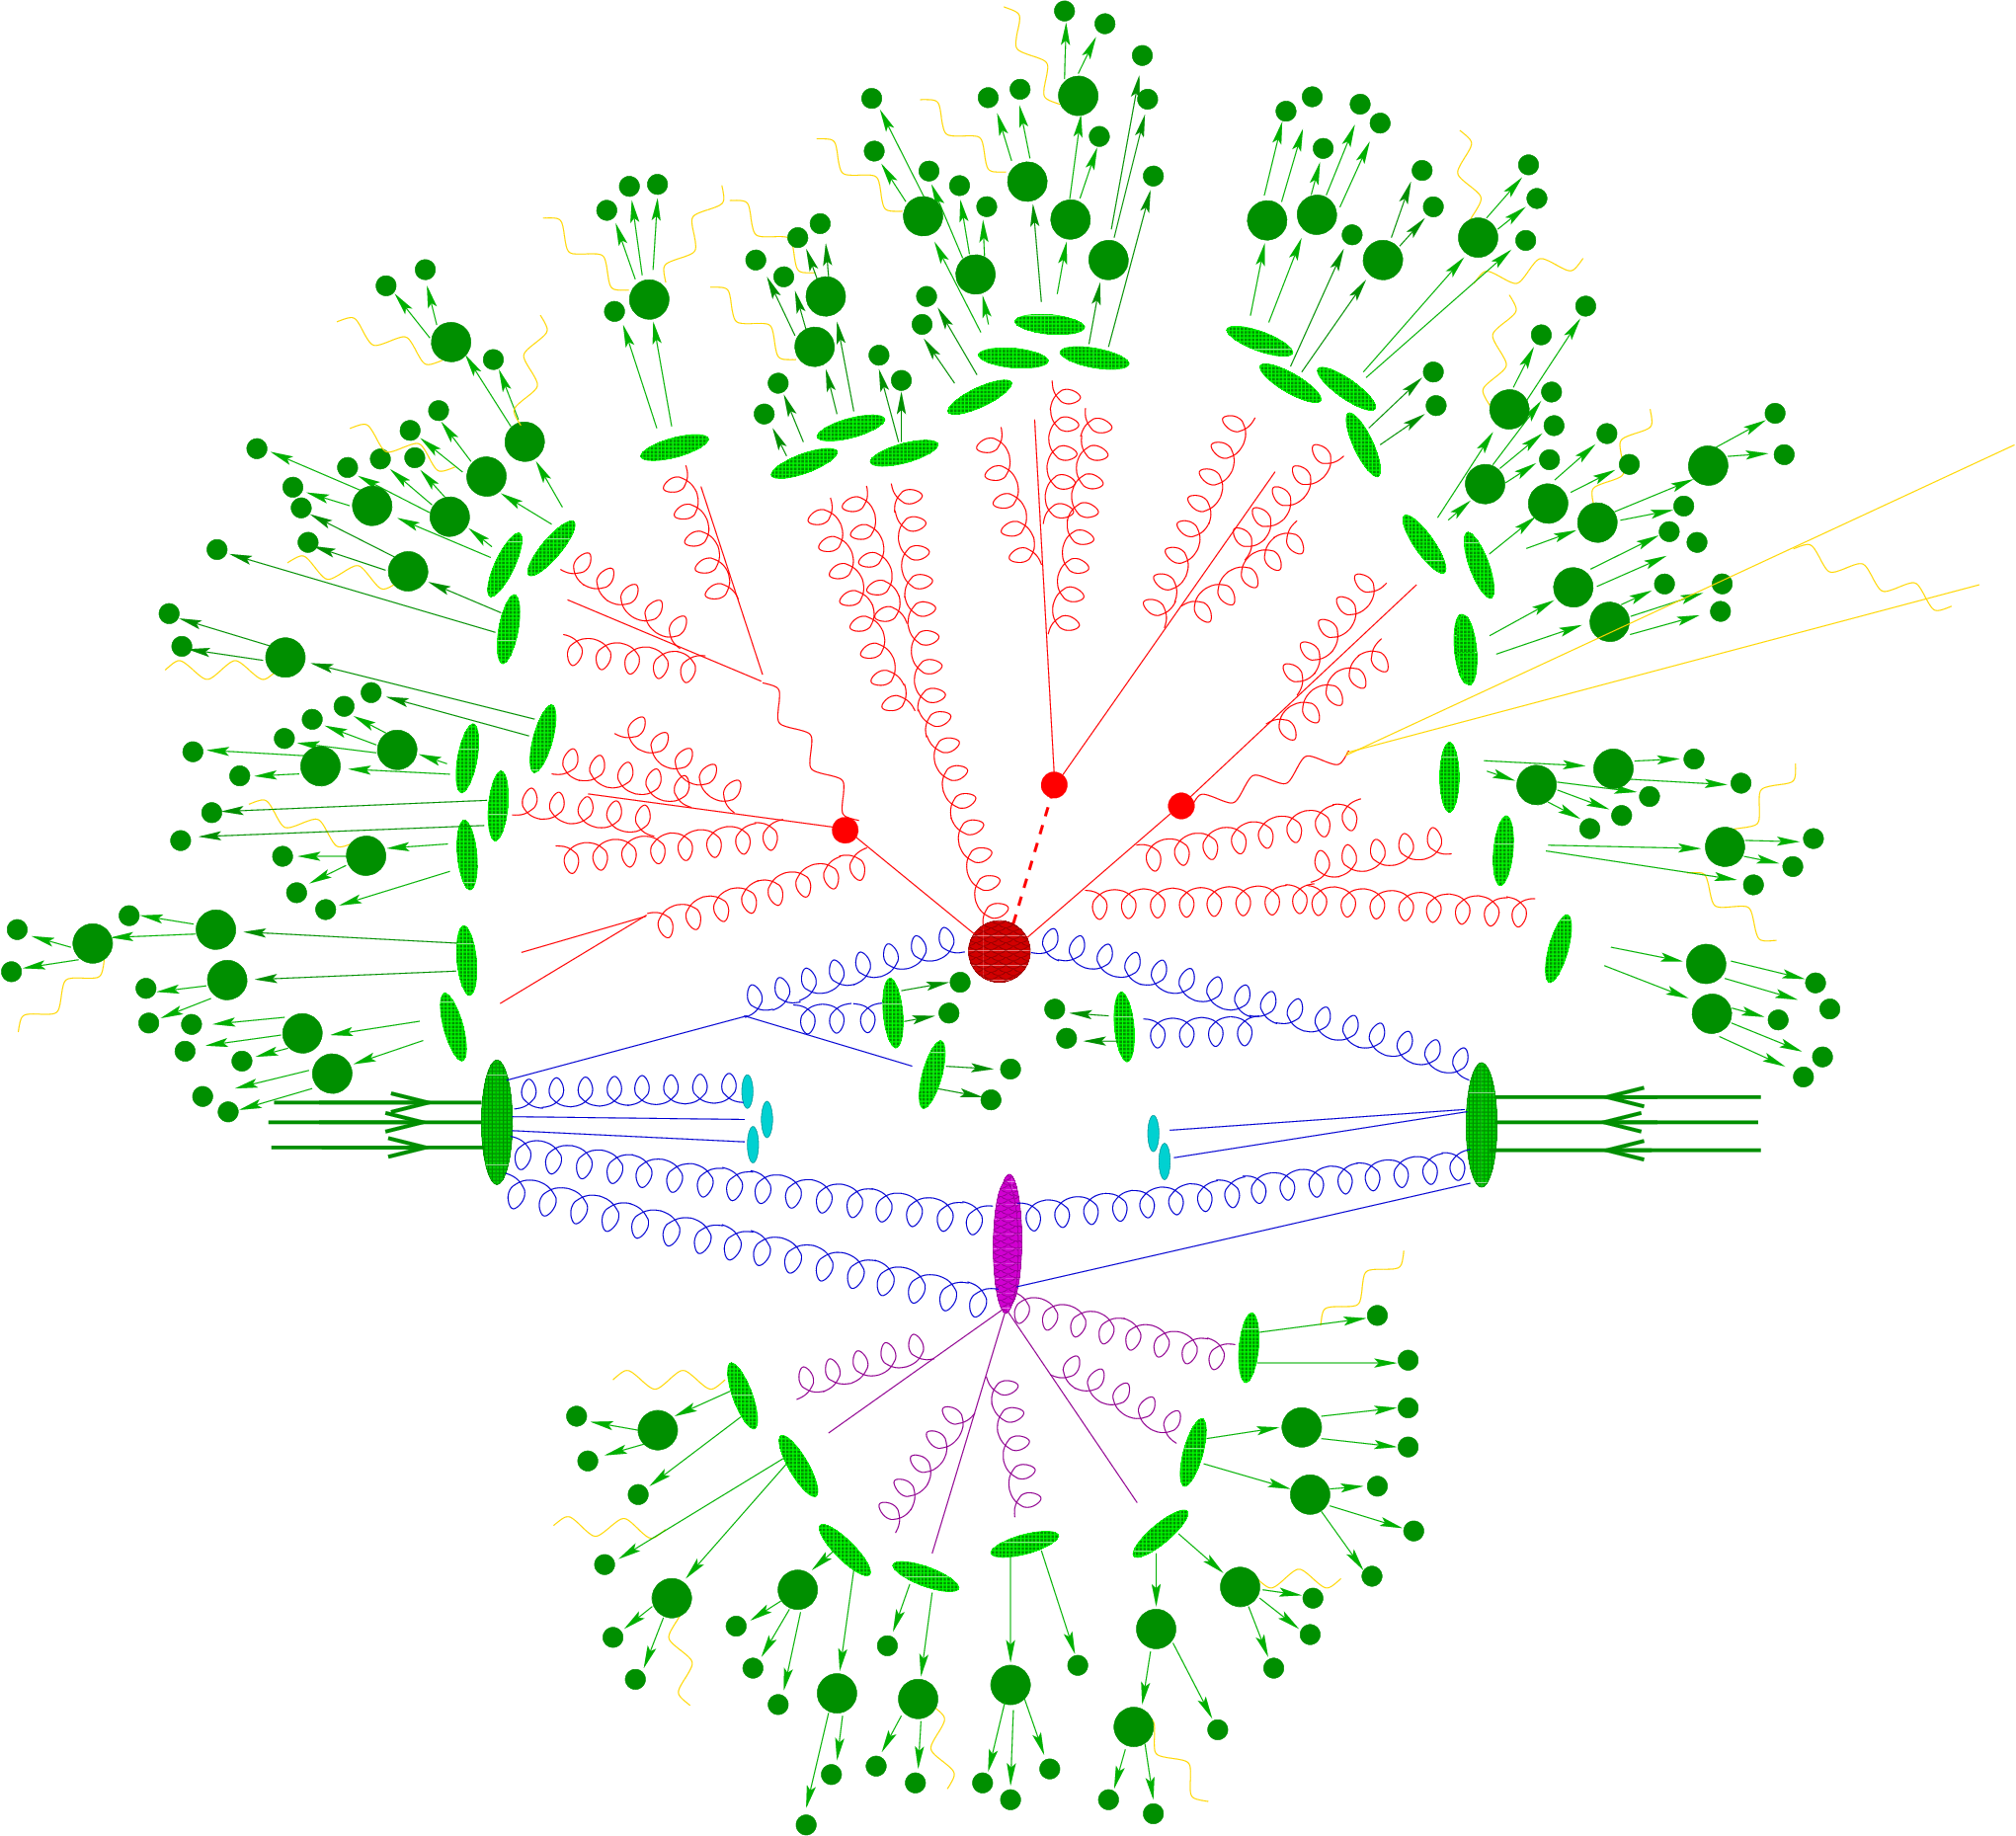
\includegraphics[width=1\textwidth]{chapters/chapter3_eventreco/images/parton-shower.png}

    \caption[Schematic of the procession of a simulated hadron-hadron collision.]{Schematic of the procession of a simulated hadron-hadron collision through hadronization. The red circle represents the matrix element, simulated by an event generator. The emitted red lines represent the bremsstrahlung radiation, which is simulated by a parton shower. The purple oval represents a secondary vertex. Hadronization is represented by the light green circles, in which hadrons are produced (dark green) as well as photon radiation (yellow)~\cite{parton-shower-sketch}.}
    \label{fig:parton-shower-sketch}
\end{figure}


\subsection{Detector Simulation}  \label{ssec:simulation} 
After hadronization, the model is a full detector-independent description of a process; next, the simulation must model how the particle will interact with the ATLAS detector. In order to do this, a component-level model of the ATLAS detector is implemented in \GEANTFOUR~\cite{geant4}, and particles are propagated through this model. The energy deposition in each detector component is calculated stochastically and output as a collection of hits. The electrical response for these hits in each detector component is simulated, and output in a format matches that from actual data collection. From this, physics objects may be reconstructed via the same methods as real data, outlined in Section~\ref{sec:reconstruction}.

While this method is the most accurate method of simulation, it is CPU-intensive. Methods of faster simulation have been developed to mitigate this problem. The \gls{AFII} simulation reduces simulation time by an order of magnitude through using FastCaloSim for calorimeter simulation~\cite{fastcalosim}. FastCaloSim uses parameterizations of electromagnetic showers to directly deposit energy rather than explicit simulation.


\section{Object Reconstruction}\label{sec:reconstruction}

Both the full simulation chain and actual data collection result in a set of hits within the ATLAS detector. Reconstruction is the method by which these hits are defined into final physics objects useful for analysis. This is performed independently for each type of signature. The following sections discuss the reconstruction of objects used in the analysis presented in this thesis. For the Higgs decays studied, the final state physics objects are a pair of photons (discussed in Section~\ref{ssec:em-signatures}) and a pair of jets (discussed in Section~\ref{ssec:jet-reco}). To account for energy losses in jets, corrections using muons (discussed in Section~\ref{ssec:muon-reco}) are applied. In addition to the objects used in this analysis, ATLAS reconstructs tau leptons and \gls{MET} (corresponding to neutrino signatures in \gls{SM} analyses, as well as a number of \gls{BSM} signatures), not discussed here.

\subsection{Electromagnetic Signatures: Electrons and Photons}\label{ssec:em-signatures} %https://arxiv.org/pdf/1908.00005.pdf

\noindent\textbf{Interaction}\\
\indent Photons and electrons interact with the \gls{LAr} calorimeter, leaving an electromagnetic signature in a group of neighboring cells known as \textit{showering}. Their reconstruction is performed in parallel due to the similarity in signature.

\gls{EM} signatures can be the result of three different sources:
\begin{itemize}
    \item Electrons: Being a charged lepton, in addition to interactions in the \gls{EM} calorimeter, electrons interact with the \gls{ID}, leaving a track that can be extrapolated to the \gls{EM} cluster.
    \item Converted Photons: Photons that pair produce electron-positron pairs in the detector prior to the calorimeter have a \gls{EM} cluster matched to a secondary vertex. The rate of photons that convert varies with $\eta$, as more detector material is traversed at higher angles. At low \abseta, about 20\% of photons convert, where above $\abseta=2.3$, up to 65\% convert~\cite{photon-electron-perf}.
    \item Unconverted Photons: Unconverted photons do not interact with the \gls{ID}, and thus are not matched to an electron track or secondary vertex.
\end{itemize}

As a result of bremsstrahlung radiation, an electron can lose a substantial portion of its energy as it traverses the detector material. In this process, the electron radiates a photon, which itself can radiate an electron-positron pair. Should these occur in the beampipe or \gls{ID}, there may be multiple track candidates from the same electron. The process by which these depositions become final analysis objects proceed in steps of cluster reconstruction, track reconstruction, supercluster reconstruction, then construction of the final analysis object.


\noindent\textbf{Cluster Reconstruction}\\
\indent The algorithm to build electron and photon candidates is a dynamic algorithm, building variable-sized clusters. This is in contrast to previous methods, which use a fixed ``sliding window'' definition~\cite{sliding-window}. The algorithm starts from a \textit{seed} cell, which is identified by a signal larger than a high signal threshold relative to underlying electronic noise, $S\sigma_{noise}$. The seed and its neighbors are added to the cell, known as a \textit{proto-cluster}. Then, all neighbor\footnote{In the same sampling layer, neighboring means cells are adjacent. In adjacent layers, neighboring cells must have overlap in the $(\eta,\phi)$ plane.} cells are scanned for a signal larger than a moderate threshold, $N\sigma_{noise}$. The subsequent neighbors of cells meeting this criteria are added to the cluster, and themselves are evaluated if they pass the moderate signal threshold, provided that they pass a cell filter defined by $P\sigma_{noise}$. In the case where two clusters have an overlapping cell, the clusters are merged. ATLAS uses default values of $S=4,N=2,P=0$ in this algorithm. The choice of $P=0$ means that no filter is applied, and candidates passing the $2\sigma_{noise}$ have all neighboring cells added to the cluster. This method of clustering is known as  \textit{topological} (topo) clustering~\cite{topo-cluster}. 

For \gls{EM} objects, only energy in the \gls{EM} calorimeter is used\footnote{In the crack in the \gls{EM} calorimeter, $1.37<|\eta|<1.63$, the presampler and scintillator between the calorimeter cryostats are used.}, denoted \gls{EM} energy. Clusters considered for must pass a \gls{EM} fraction ($f_{\text{EM}}$) criteria, in which the \gls{EM} energy must be greater than 50\% of the total cluster energy. This cut rejects $\sim$60\% of pile-up clusters with no affect on true electron topo-clusters. Clusters passing this criteria are known as \gls{EM} topo-clusters.

\noindent\textbf{Track Reconstruction}\\ %https://arxiv.org/pdf/1902.04655.pdf
\indent Tracks are constructed out of hits within the \gls{ID}, in which three dimensional space-points are constructed out of clusters. Three sets of space-points are formed into track seeds, which then undergo stages of pattern recognition, ambiguity resolution, and \gls{TRT} extension. Track candidates with $\pt > \unit{400}{\MeV}$ are fit with the ATLAS Global $\chi^2$ fitter~\cite{chi-2-fitter}.

For tracks with at least four silicon hits that match to an \gls{EM} cluster, a secondary fit is performed using a Gaussian-sum filter~\cite{gaussian-sum-filter}. This filter is is a generalization of the Kalman filter~\cite{kalman-filter}, taking into account non-linearities resulting from bremsstrahlung radiation. The separation between the cluster barycenter and the position of the track extrapolated from the perigee to the calorimeter must satisfy\footnote{This requirement is asymmetric because clusters can measure energy from radiated photons that tracks miss.} $|\eta_{cluster} - \eta_{track}| < 0.05$, and $-0.10 < q \cdot (\phi_{track}-\phi_{cluster}) < 0.05$ for reconstructed track charge, $q$.

%https://arxiv.org/pdf/1908.00005.pdf

If multiple tracks are matched to a cluster, they are ranked. First, priority is given to tracks with pixel hits over those with just \gls{SCT} hits. Second, tracks are ordered in \Dr to the cluster. If multiple tracks have small \Dr differences, then the track with the most pixel hits is selected. 


\noindent\textbf{Supercluster Reconstruction}\\ 
\indent The object ultimately defined as an electron or photon is a supercluster, which is a grouping of topo-clusters.  Superclusters are formed in a two-stage process.

First, topo-clusters are tested for use as a seed for the supercluster. Topo-clusters are sorted by \et, then sequentially tested to be seed candidates. An electron seed candidate must have $\et \geq \unit{1}{\GeV}$ and a matching track; a photon seed must have $\et \geq \unit{1.5}{\GeV}$. 

Second, the topo-clusters near the identified seed are selected to be added to the supercluster. These extra topo-clusters, called satellite clusters, can arise from either splitting or through bremsstrahlung radiation. A window of $\Delta \eta \times \Delta \phi = 0.075 \times 0.125$ around the barycenter is considered. A wider window of $\Delta \eta \times \Delta \phi = 0.125 \times 0.300$ is used for electrons if the best-matched track for the seed cluster is the same best-matched track for the satellite cluster. For photons that have converted, a cluster is added if its best-matched track belongs to the conversion vertex matched to the seed. The supercluster reconstruction logic is shown in Figure~\ref{fig:supercluster-reco}.

\begin{figure}[h]
    \centering
    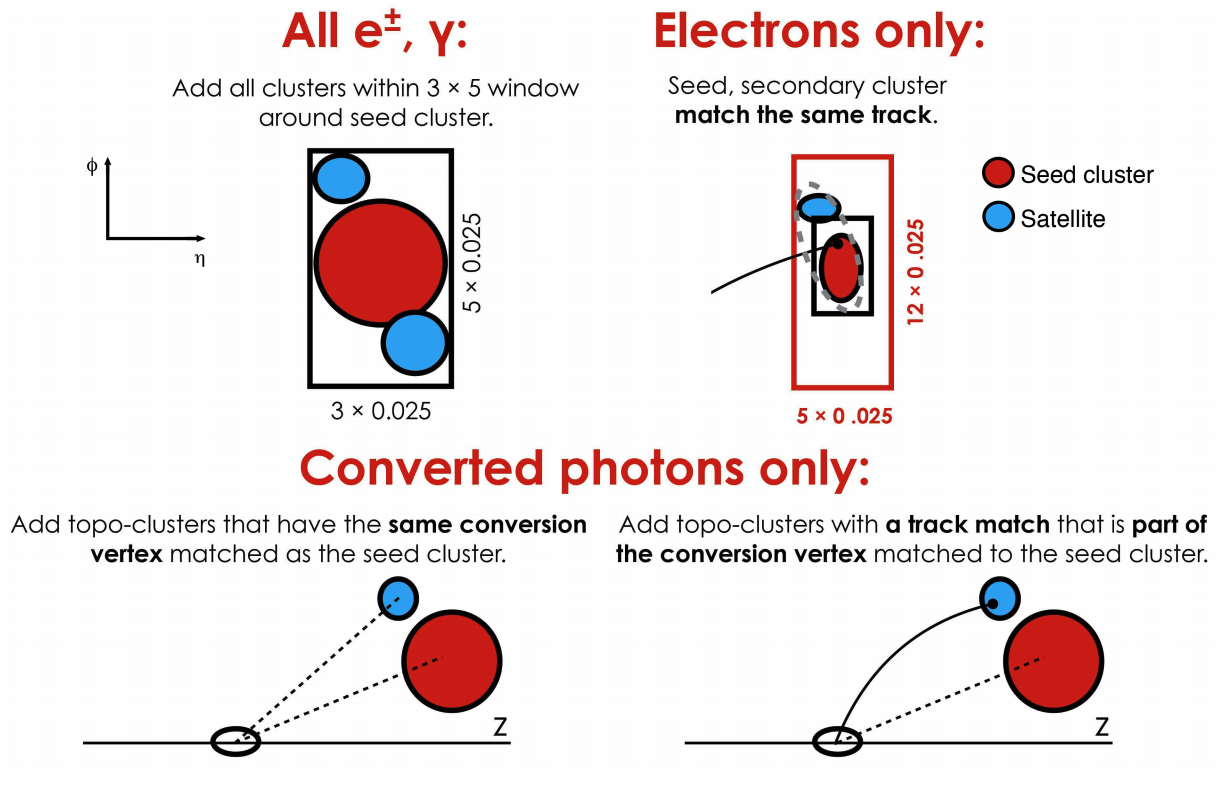
\includegraphics[width=.90\textwidth]{chapters/chapter3_eventreco/images/supercluster-formation.png}
    \caption[Pictorial representation of supercluster algorithm for \gls{EM} objects]{Pictorial representation of supercluster algorithm for \gls{EM} objects~\cite{photon-electron-perf}. The resolution of $0.025$ is due to the granularity of the \gls{EM} calorimeter.}
    \label{fig:supercluster-reco}
\end{figure}


\begin{figure}[!htb]
    \centering
    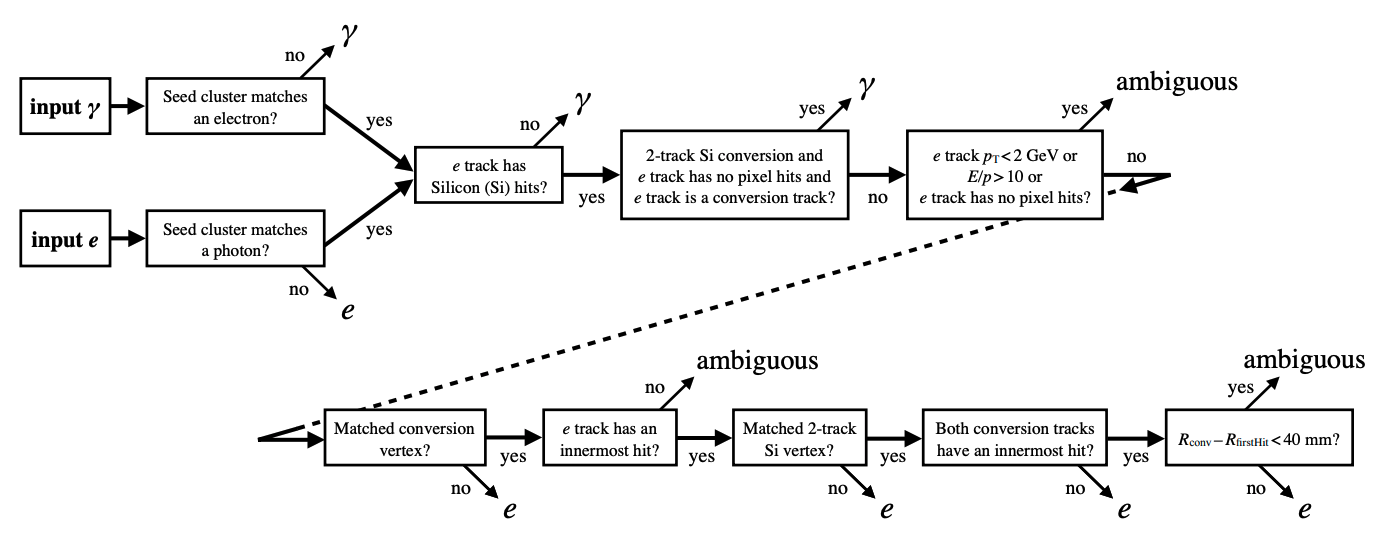
\includegraphics[width=1\textwidth]{chapters/chapter3_eventreco/images/egamma-amb.png}

    \caption[Logic flowchart for superclusters that are reconstructed as both an electron and a photon]{Logic flowchart for superclusters that are reconstructed as both an electron and a photon~\cite{photon-electron-perf}.}
    \label{fig:ambiguity-logic}
\end{figure}


\begin{figure}[!htb]
    \centering
    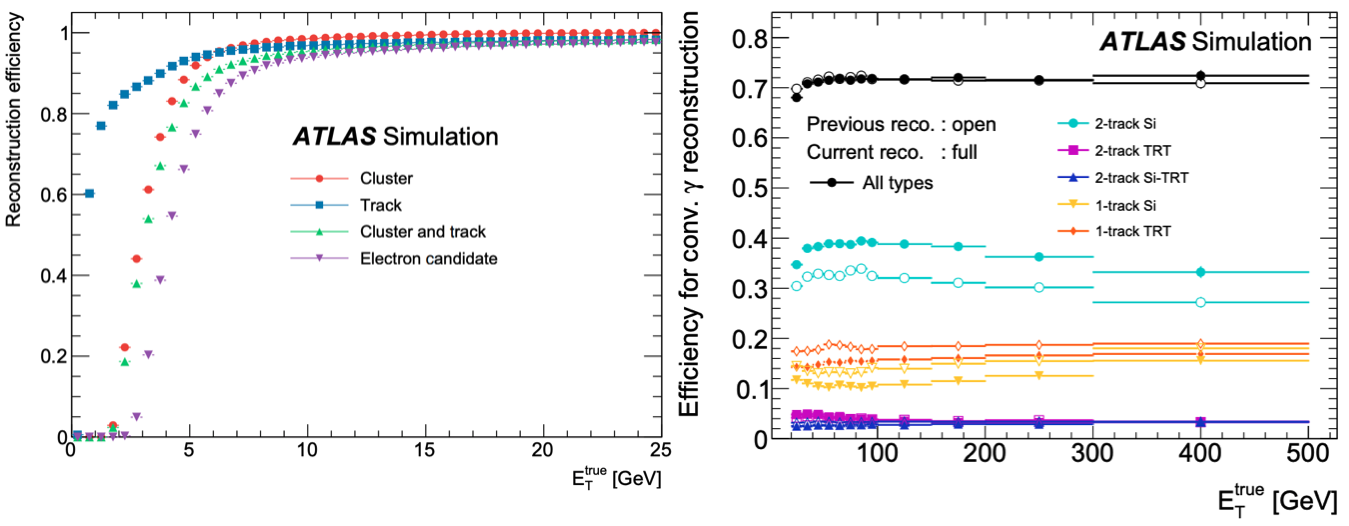
\includegraphics[width=1\textwidth]{chapters/chapter3_eventreco/images/combined-efficiency.png}

    \caption[The reconstruction efficiency as a function of \et for electrons and converted photons]{The reconstruction efficiency as a function of \et for clusters, track, cluster and track, and electrons (left) and the various photon conversion types (right)~\cite{photon-electron-perf}.}
    \label{fig:reco-eff}
\end{figure}

\noindent\textbf{Analysis Objects}\\ 
\indent Once superclusters are constructed, they make up the final analysis objects, but due to the logic of supercluster formation, a seed could be both an electron and photon candidate. In these cases, after calibration and positron correction, the logic shown in Figure~\ref{fig:ambiguity-logic} is applied. In cases denoted ambiguous, both a photon and electron are formed, and these are marked as ``ambiguous'' for analysis-specific requirements. The electron and converted photon reconstruction efficiency is shown in Figure~\ref{fig:reco-eff} as a function of truth \et.

\subsection{Jets}\label{ssec:jet-reco}
As discussed in Section~\ref{ssec:fermions}, strongly interacting particles cannot exist independently due to color confinement. Due to this, partons created in $pp$ collisions shower, a process where they produce additional strongly interacting particles through splitting and radiation. This creates a proliferation of nearly collinear subsequent partons. Ultimately, once they've reached a sufficiently low energy, about $\unit{1}{\GeV}$, they hadronize in order to create a colorless state, such as mesons or baryons that deposit energy into the calorimeters. This spray of interactions all proceeding in the same general direction as the initial parton is known as a ``jet.''

In principle, jets can be built from any set of 4-vector objects. The standardized jet definition~\cite{jet-standardization} requires that jets be:
\begin{itemize}
    \item Simple to implement in both experimental analysis and theoretical calculation.
    \item Defined at any order of perturbation theory, and yield a finite cross-section.
    \item Yield a cross-section relatively insensitive to hadronization.
\end{itemize}

For this work, they are constructed via topological clusters. The topological clustering logic described in detail in~\ref{ssec:em-signatures} can also be applied to the hadronic calorimeter and jets can be formed out of these topo-clusters or \gls{EM} topo-clusters~\cite{topo-cluster}. Two classes of jet definitions exist. The first is cluster-based, which defines the jet by combining sets of four-vector objects until the distance between objects surpasses a stopping condition. The second is cone-based, which define jets as the sum of momenta within a defined radius, realizing jets as energy flow in a specified direction. ATLAS uses one such cone-based algorithm, known as the Anti-$k_t$ algorithm~\cite{anti-kt}. The cone is built from topological clusters using a fixed radius\footnote{In analyses that probe high mass regimes, two jets may be overlapping and merge to produce one single large radius jet. This is known as a ``boosted'' topology, where the radius parameter is typically $R=1.0$. The presented analysis is not sensitive at high mass, thus such topologies are not considered.}, $R=0.4$.


Since all fragmenting strongly interacting particles appear as jets in the detector, an important process is \textit{flavor tagging}, which aims to classify the type of particle that produced a given jet. Paramount to the presented analysis is the process of $b$-tagging\footnote{In addition to $b$-tagging, ATLAS has also produced discriminators for charm jets ($c$-tagging).}, the method of classifying jets which come from $b$-quarks. There are several algorithms to perform this classification, notably a \gls{BDT} named MV2~\cite{mv2-dl1} and a feed-forward deep \gls{NN}\footnote{See Appendix~\ref{app:MVA} for an explanation of these multivariate techniques.} known as DL1~\cite{mv2-dl1}. From this score, $b$-tagging working points are established and calibrated based on their identification efficiency. 


\subsection{Muons}\label{ssec:muon-reco}
%http://cds.cern.ch/record/2139897/files/arXiv:1603.05598.pdf

Muons are a minimum-ionizing particles, leave very little energy in the calorimeter, and are not stopped by any of the material in ATLAS. Thus, muons are reconstructed using a combination of track-based information from the \gls{ID} and the \gls{MS}. In the \gls{ID} tracks for muons are identical to other charged particles, outlined in Section~\ref{ssec:em-signatures}. In the \gls{MS}, each detector region (i.e. \glspl{MDT}, \glspl{CSC}, etc.), builds track segments from aligned hits in the bending plane of the detector, found via a Hough transform~\cite{hough-transf}. Track candidates are formed by fitting together hits from different track segments via a combinatorial search outlined in Reference~\cite{muon-reco}. Then an overlap removal algorithm finds the optimum track assignment. Hits are fitted with a global $\chi^2$ fit. Afterward, a hit recovery and subsequent track refit are performed if necessary.

Ultimately four muon types are defined~\cite{muon-reco}:
\begin{itemize}
    \item Combined (CB) muon: Tracks reconstructed in the \gls{ID} are formed into a combined track using a global refit incorporating hits from both subdetectors.
    \item Segment-tagged (ST) muon: An \gls{ID} track is extrapolated to a local track segment in the \gls{MDT} or \gls{CSC}, accounting for muons that only cross one layer of \gls{MS} chambers.
    \item Calorimeter-tagged (CT) muon: An \gls{ID} track matched to a energy deposit in the calorimeter compatible with a minimum-ionizing particle. This muon type compensates for portions of the \gls{MS} that are only partially instrumented, near $\abseta \approx 0$.
    \item Extrapolated (ME) muons: These use only track information from the \gls{MS}, where parameters must be loosely in agreement with the location of the \gls{IP}. ME muons are useful for acceptance in $2.5 < \abseta < 2.7$, which is uncovered by the \gls{ID}.
\end{itemize}


From these muons, four selections are created (\textit{loose}, \textit{medium}, \textit{tight}, and \textit{high-\pt}). These are defined based on varying requirements on the type of muon considered, number of hits, $\chi^2$ fit, $\eta$, $q/p$ significance, and \pt. The efficiencies for the \textit{loose} and \textit{medium} selections are $>98\%$, and the \textit{tight} selection ranges from $90\%$ to $98\%$ efficient. Figure~\ref{fig:muon-eff} shows these efficiencies as a function of $\eta$.


\begin{figure}[h]
    \centering
    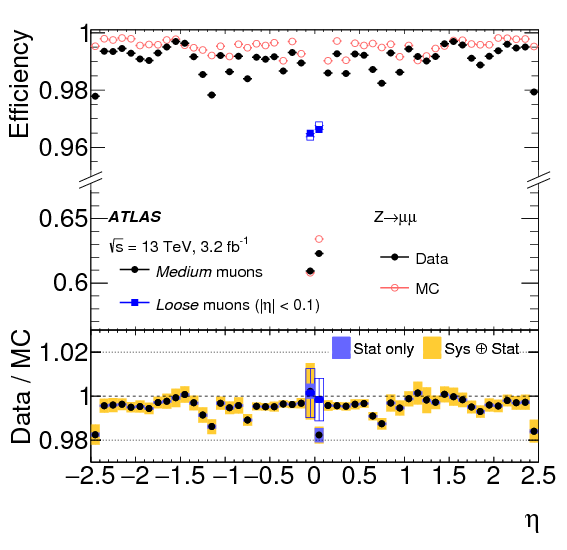
\includegraphics[width=.48\textwidth]{chapters/chapter3_eventreco/images/muon-medium.png}
    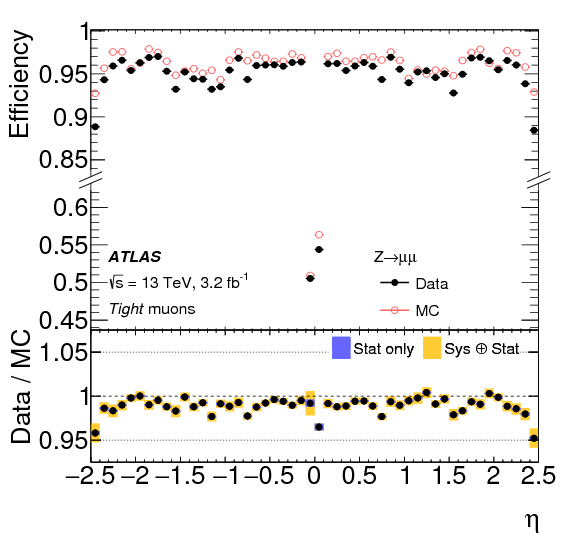
\includegraphics[width=.48\textwidth]{chapters/chapter3_eventreco/images/muon-tight.png}

    \caption[The reconstruction efficiency for \textit{loose} and \textit{tight} muons with $\pt >\unit{10}{\GeV}$ as a function of $\eta$.]
    {The reconstruction efficiency for muons with $\pt >\unit{10}{\GeV}$ as a function of $\eta$. The left panel shows the \textit{loose} selection, the right shows the \textit{tight} selection~\cite{muon-reco}.}
    \label{fig:muon-eff}
\end{figure}
